\documentclass{beamer}

\usepackage{beamerthemesplit}
\usepackage{verbatim}

\usetheme{Pittsburgh}
%\usecolortheme{seagull}
%\usecolortheme{seahorse}
\usecolortheme{beaver}

\usefonttheme{serif}

%\DeclareGraphicsExtensions{.pdf,.png,.jpg}

\newcommand{\snT}{$(S/N)_{\textrm{size}}$}
%\newcommand{\snT}{$\left( \frac{S}{N}\right)_{\textrm{size}}$}
\newcommand{\snflux}{$(S/N)_{\textrm{flux}}$}
%\newcommand{\snflux}{$\left( \frac{S}{N}\right)_{\textrm{flux}}$}

\newcommand{\lensfit}{\texttt{LENSFIT}}
\newcommand{\numba}{\texttt{Numba}}
\newcommand{\python}{\texttt{Python}}
\newcommand{\ngmix}{\texttt{ngmix}}
\newcommand{\shear}{{\bf g}}

\title{Dark Energy Survey at BNL}
\author{Erin Sheldon}
\institute{Brookhaven National Laboratory}
\subtitle{DOE Institutional Review of the BNL HEP Research Program}

% http://texblog.net/latex-archive/plaintex/beamer-footline-frame-number/
% to add the page (frame ) number and not screw up the bottom line
% works for split themes?
\expandafter\def\expandafter\insertshorttitle\expandafter{%
      \insertshorttitle\hfill%
        \insertframenumber\,/\,\inserttotalframenumber}


\begin{document}

\frame{\titlepage}

%\section{Dark Energy Survey at BNL}

\frame
{
    \frametitle{Dark Energy Survey}

    \fontsize{9}{0.8\baselineskip}
    \begin{columns}
        \begin{column}{0.5\textwidth}    
            \begin{itemize}
                \item Imaging survey of 5000 square degrees in the 
                    southern sky (CTIO) through 5 optical filters.
                \item Study Dark Energy using weak lensing, galaxy clusters, supernovae
                    and large scale structure.
                \item First Light Fall 2012
                \item Survey Start Aug. 31 2013
                \item First year is complete, analyzing data now.
            \end{itemize}
        \end{column}
        \begin{column}{0.5\textwidth}
            \includegraphics[width=\textwidth]{ctio_blanco_crew_2013Oct-19-contrast.jpg}
        \end{column}
    \end{columns}
}

\frame
{
    \frametitle{Dark Energy Survey at BNL}

    %\fontsize{9}{0.9\baselineskip}
    \begin{columns}
        \begin{column}{0.5\textwidth}
            \begin{itemize}
                \item Erin Sheldon
                \begin{itemize}
                    \item Weak lensing shear estimation
                    \item Multi-epoch image processing
                    \item Mass measurement of galaxy clusters
                \end{itemize}
                \item Andres Plazas
                \begin{itemize}
                    \item CCD characterization
                    \item Astrometric \& photometric residuals
                    \item ``tree rings''
                    \item ``glowing edges''
                    \item Mass measurement of galaxy clusters
                \end{itemize}

            \end{itemize}
        \end{column}
        \begin{column}{0.5\textwidth}
            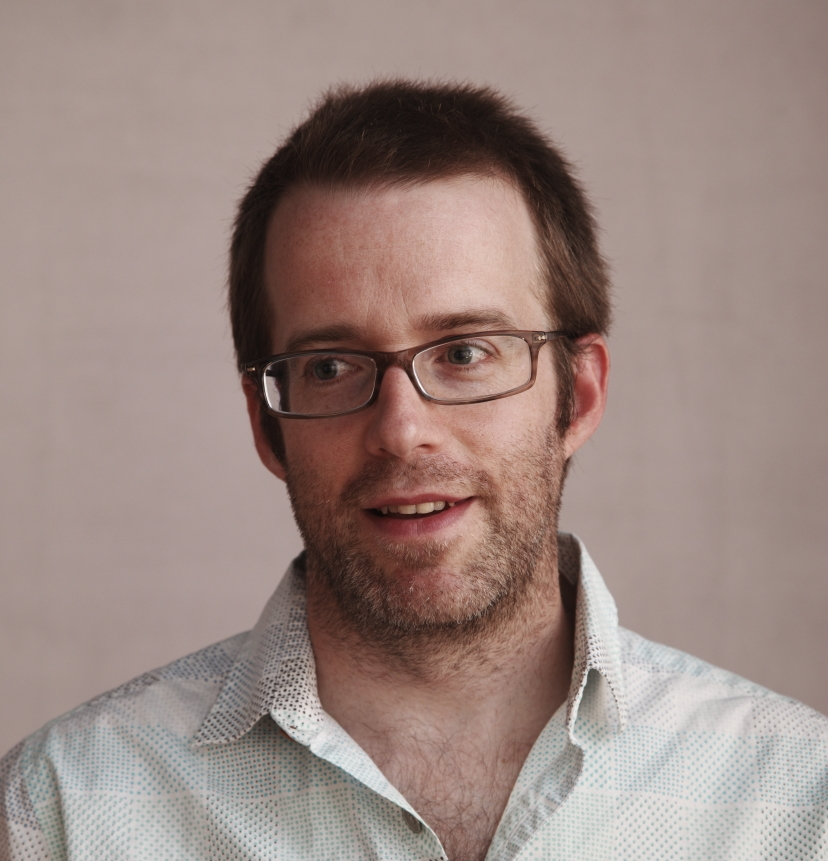
\includegraphics[width=100px]{me-head1-crop.jpg}
            \newline
            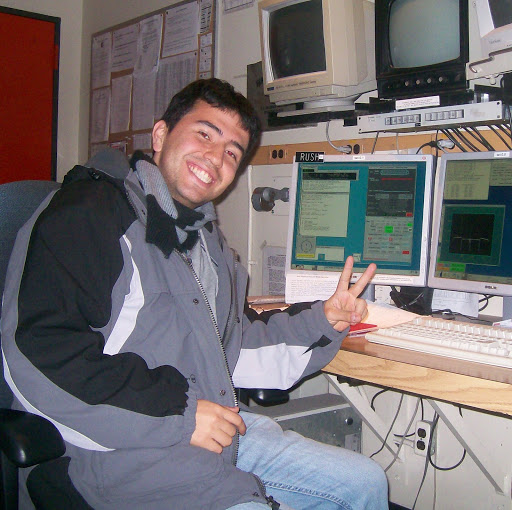
\includegraphics[width=100px]{plazas-penn.jpg}
        \end{column}
    \end{columns}

}
%                \item Erin Sheldon {\bf associate member and builder}; data rights for
%                    himself, postdoc, students.
%                \item Anders Plazas postdoc working on characterization of detector
%                    effects and weak lensing.

%\frame
%{
%    \frametitle{Oct. 2013 DES Observing Run}
%
%    \includegraphics[width=\textwidth]{ctio_blanco_crew_2013Oct-13-contrast.jpg}
%}
%\frame
%{
%    \frametitle{Sept. 2013 DES Observing Run}
%
%    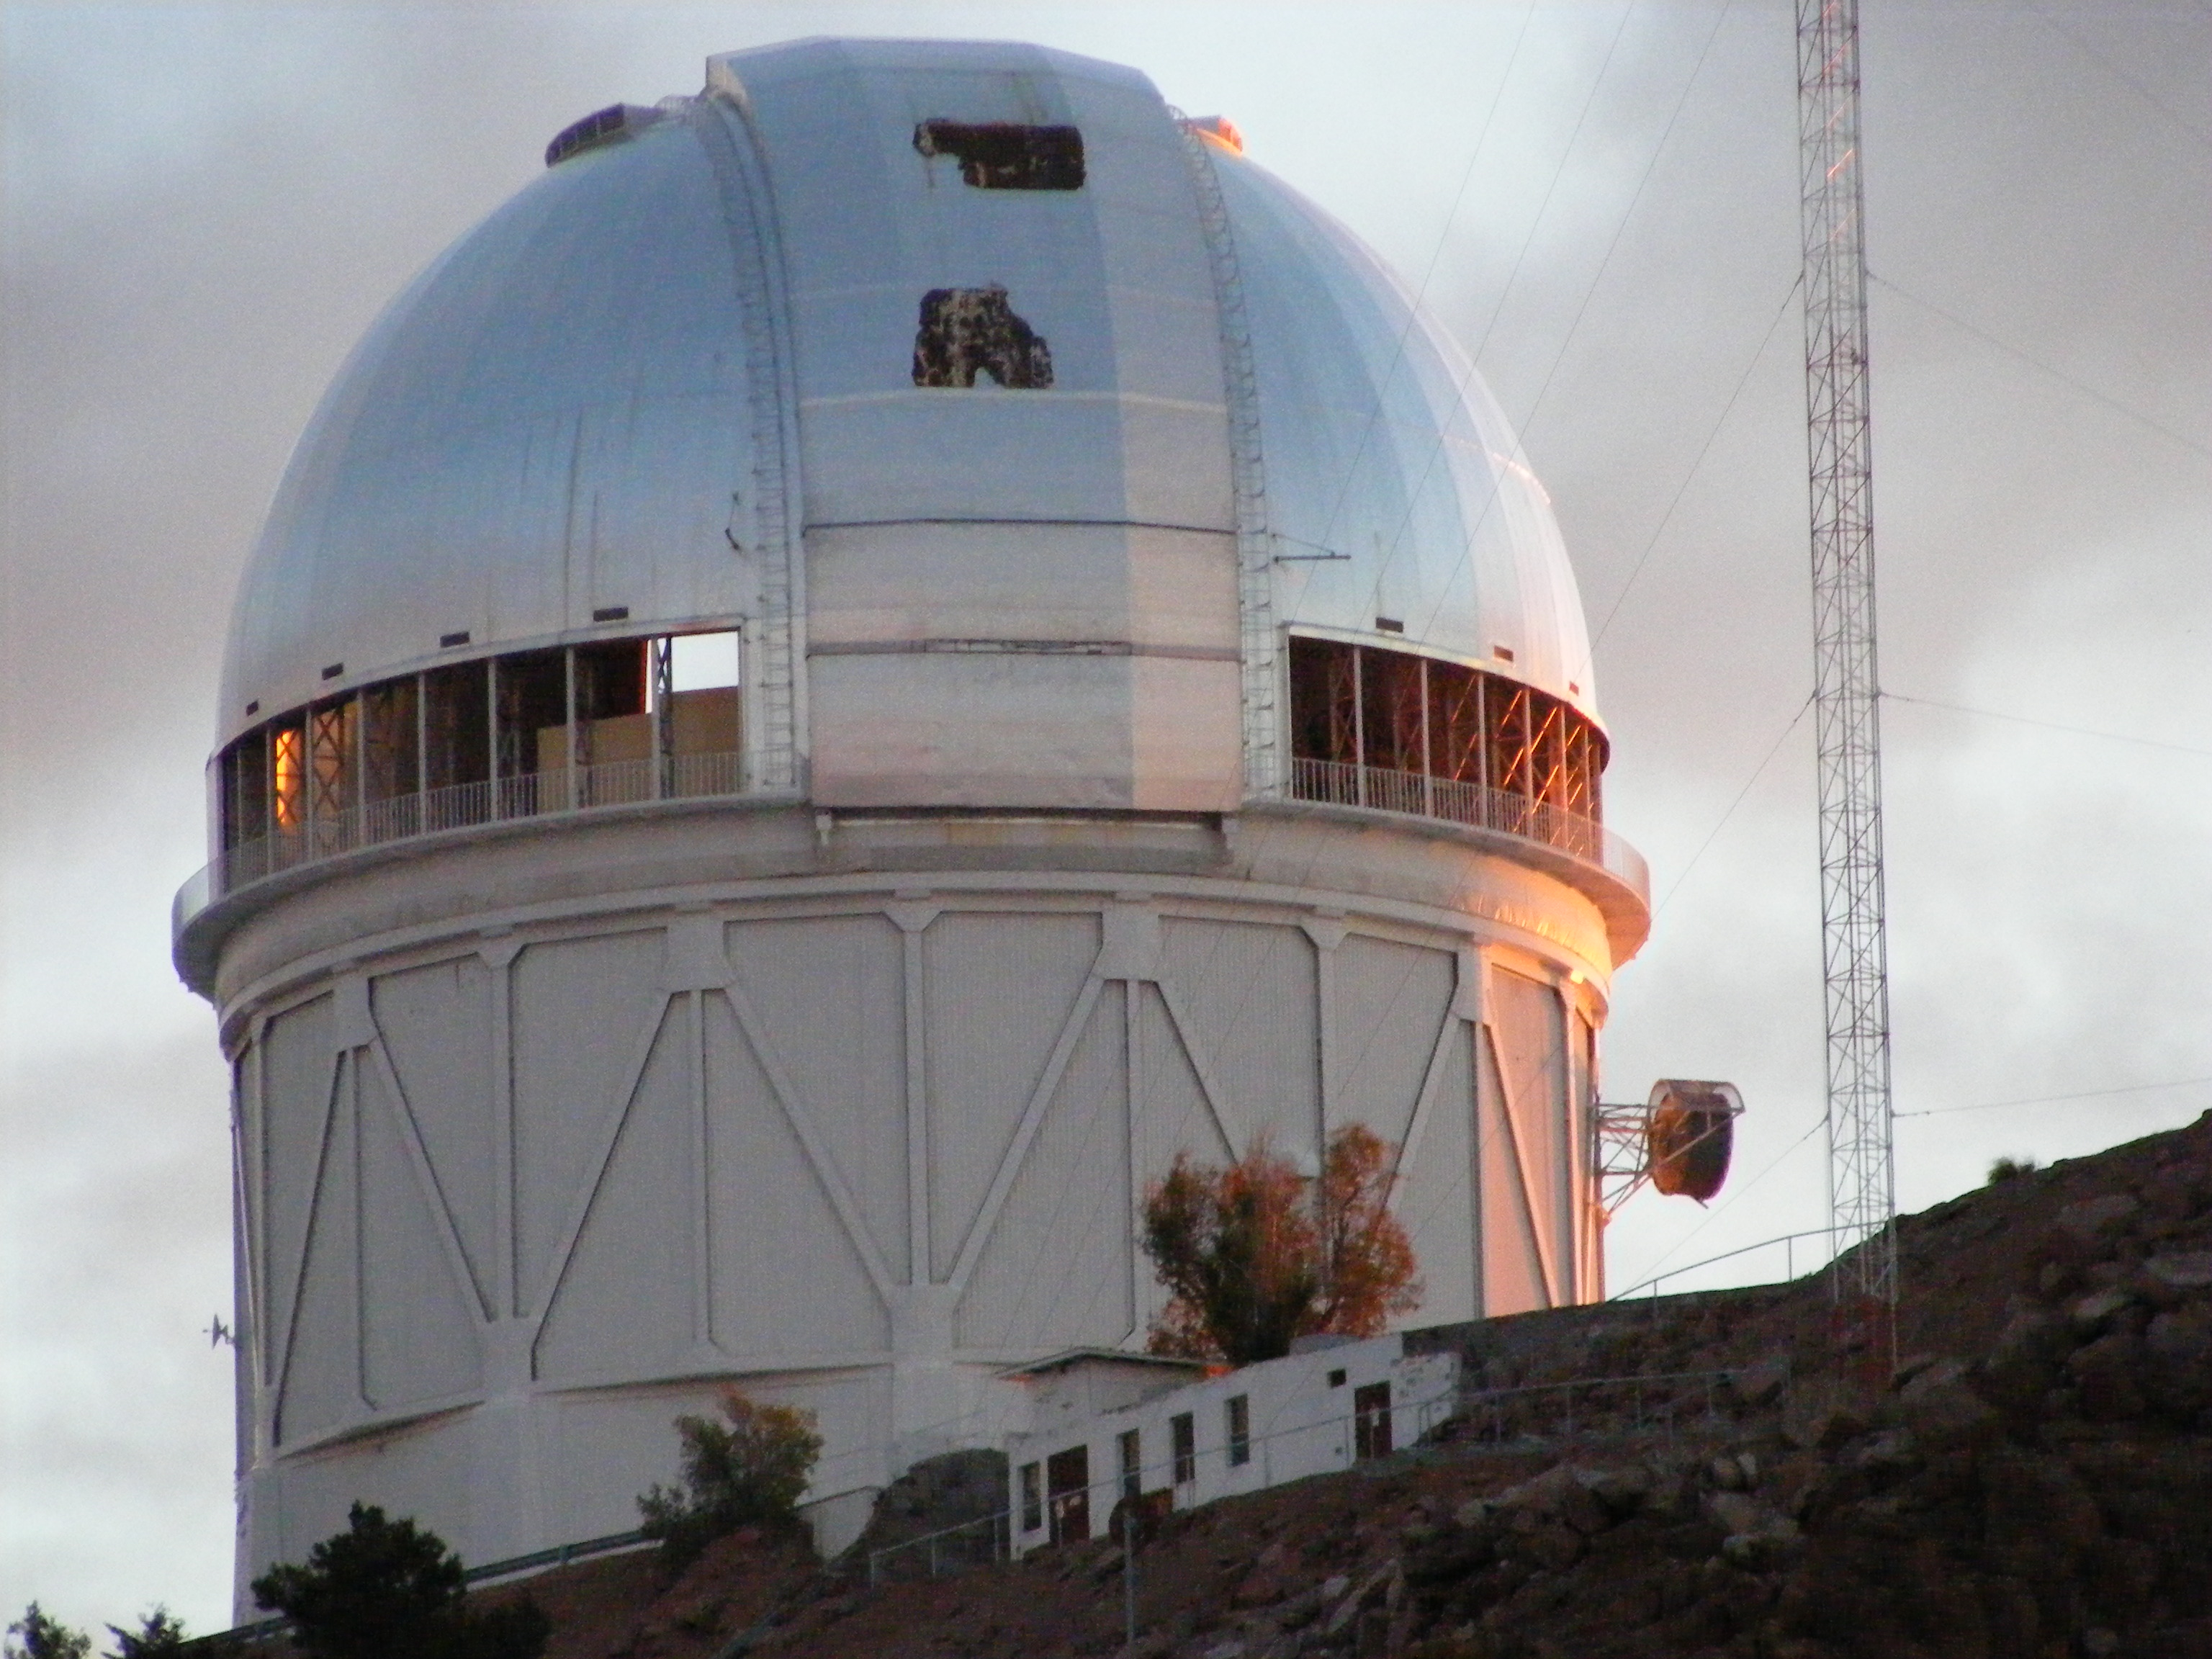
\includegraphics[width=0.5\textwidth]{plazas-blanco-ctio.jpg}
%    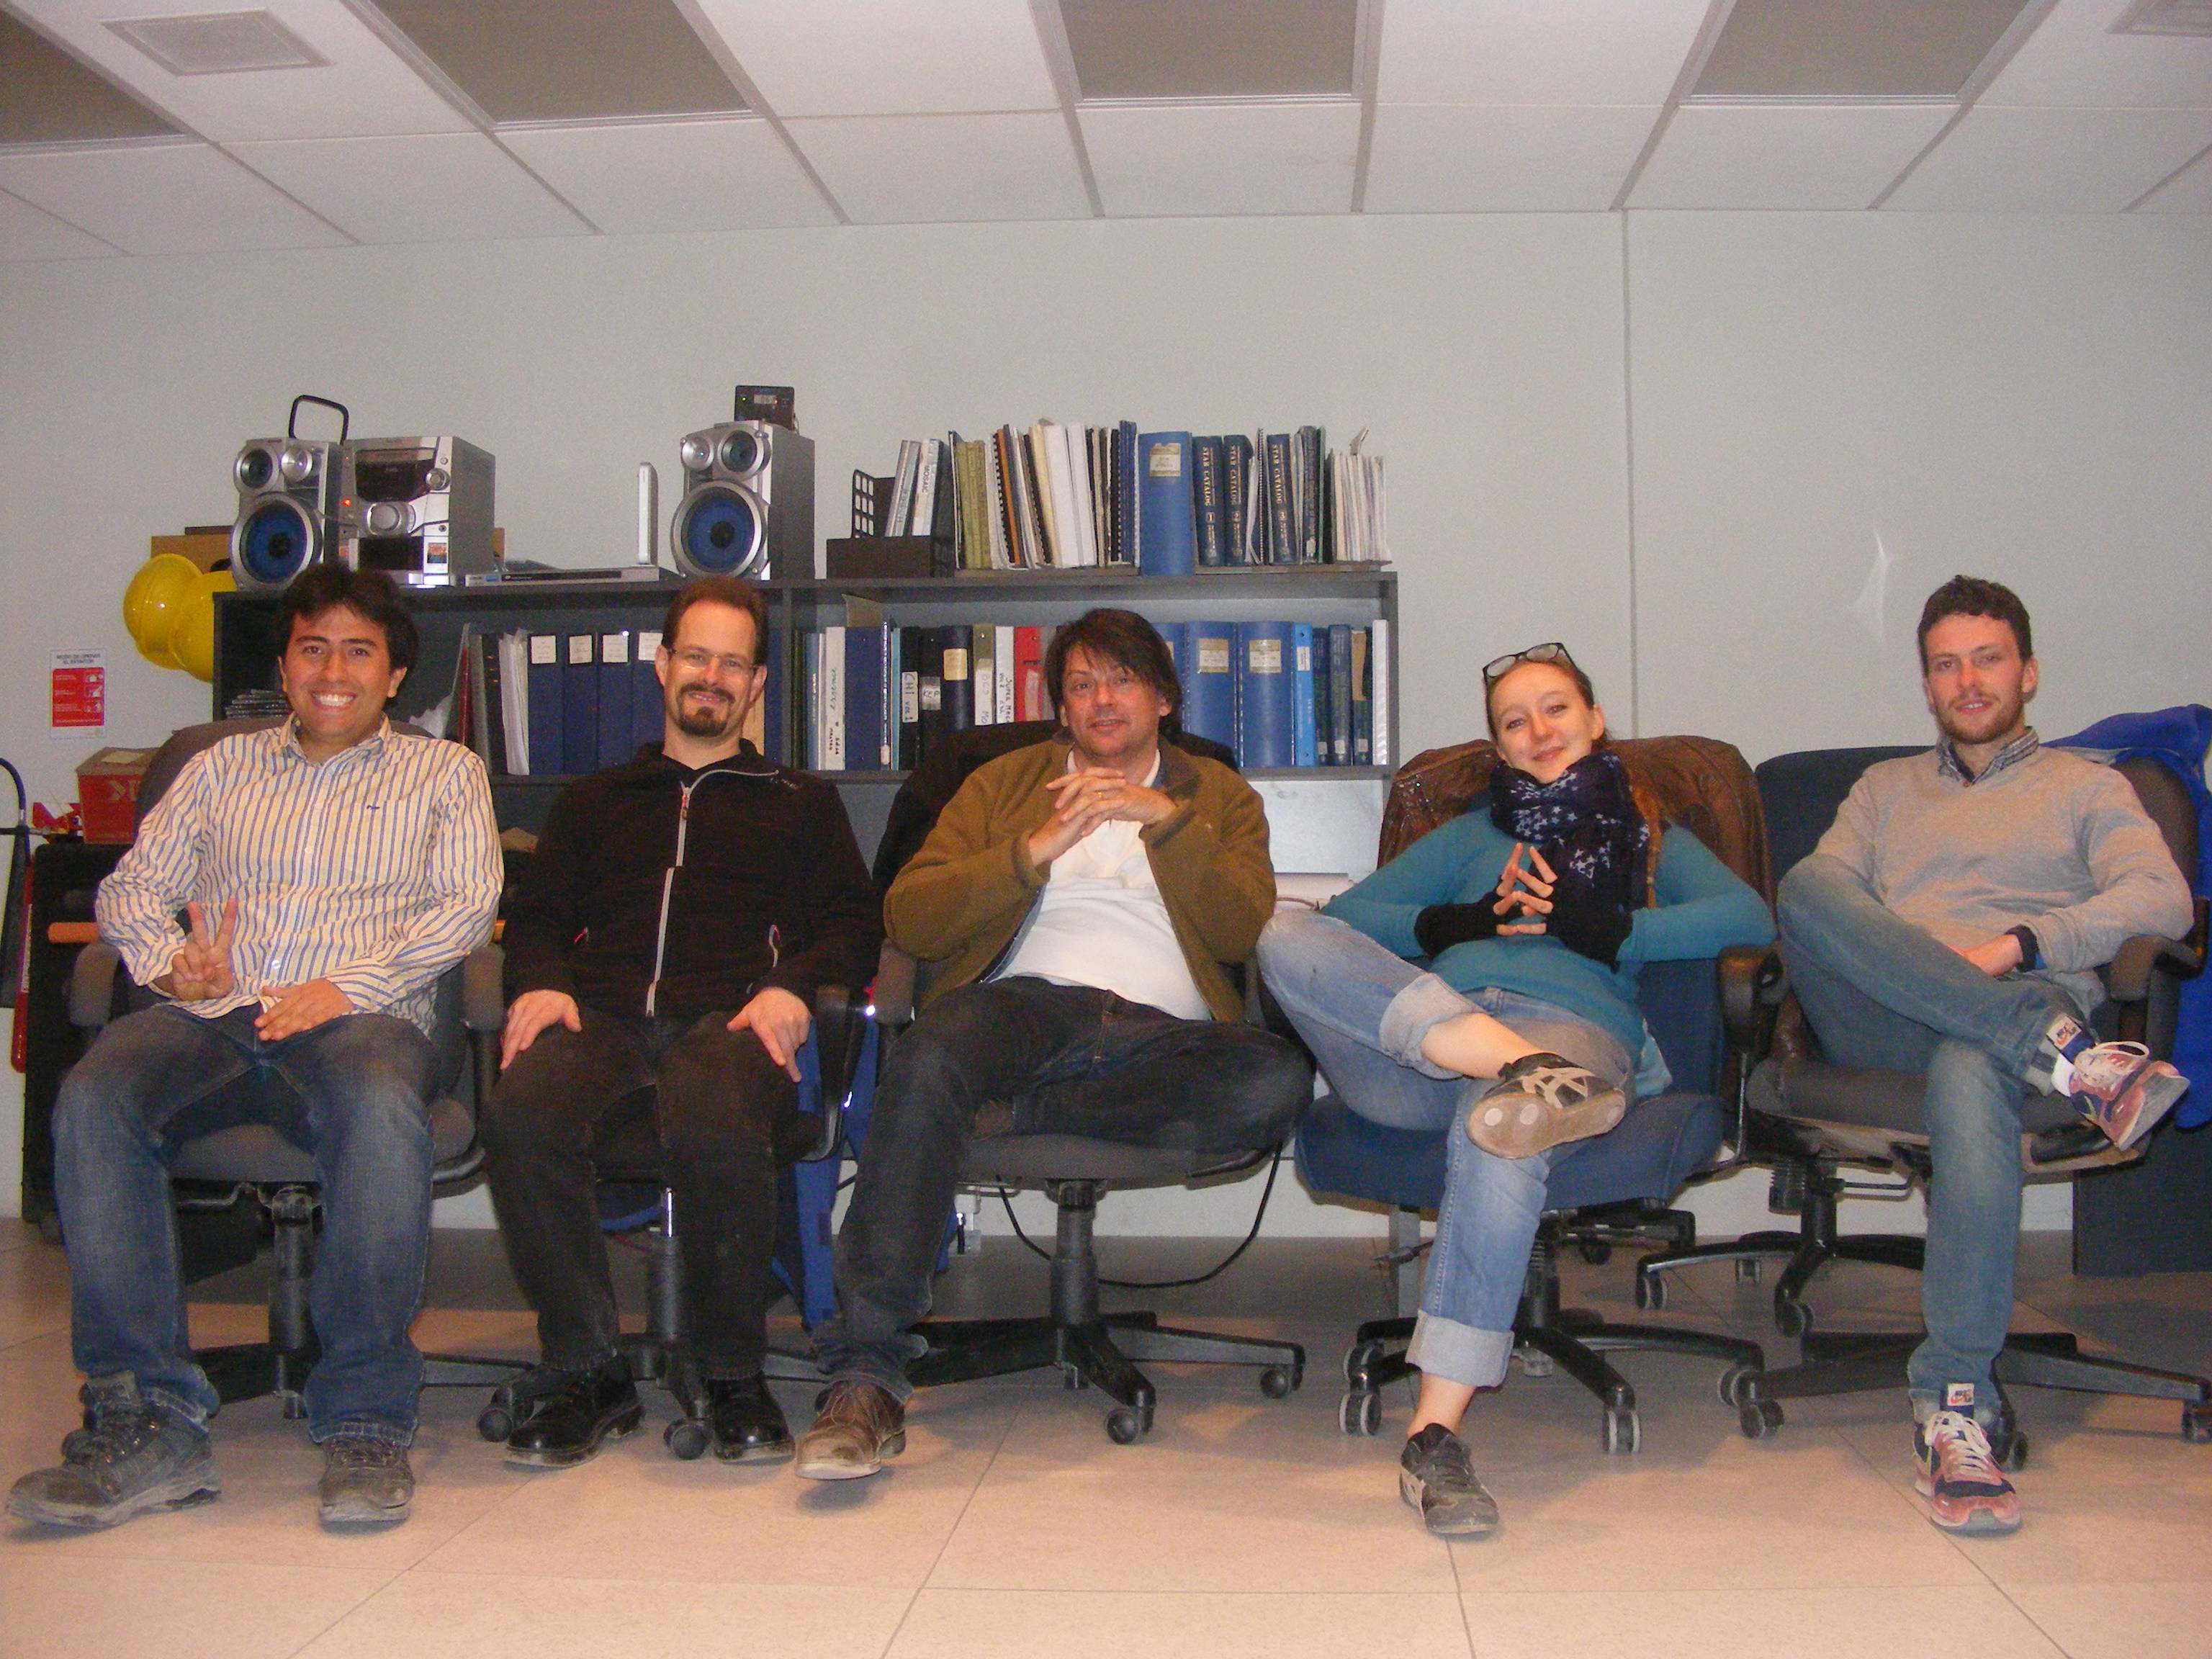
\includegraphics[width=0.5\textwidth]{plazas-group-ctio.jpg}
%}


\frame
{
    \frametitle{Erin Sheldon: Bayesian Lensing Shear Measurement}

    \begin{itemize}
        \item Theoretical work by Bernstein \& Armstrong (2014)
        \item New shear method that promises to eliminate noise-related biases.
        \item E.S. provided the first implementation.
        \item Submitted to journal arXiv:1403.7669
    \end{itemize}
}

\frame
{
    \frametitle{Erin Sheldon: Bayesian Lensing Shear Measurement}

    \fontsize{9}{0.8\baselineskip}
    \begin{columns}
        \begin{column}{0.4\textwidth}
            \begin{itemize}

                \item Figure: Fractional error in the shear for simulated
                    galaxies (exponential disk, dev. profiles) near
                    smallest usable {\it observed} size
                    fwhm/fwhm$_{\textrm{psf}}$ = 1.2.

                \item Light Grey: DES requirements
                \item Dark Grey: LSST requirements
                \item Running on DES data
            \end{itemize}
        \end{column}
        \begin{column}{0.6\textwidth}
            %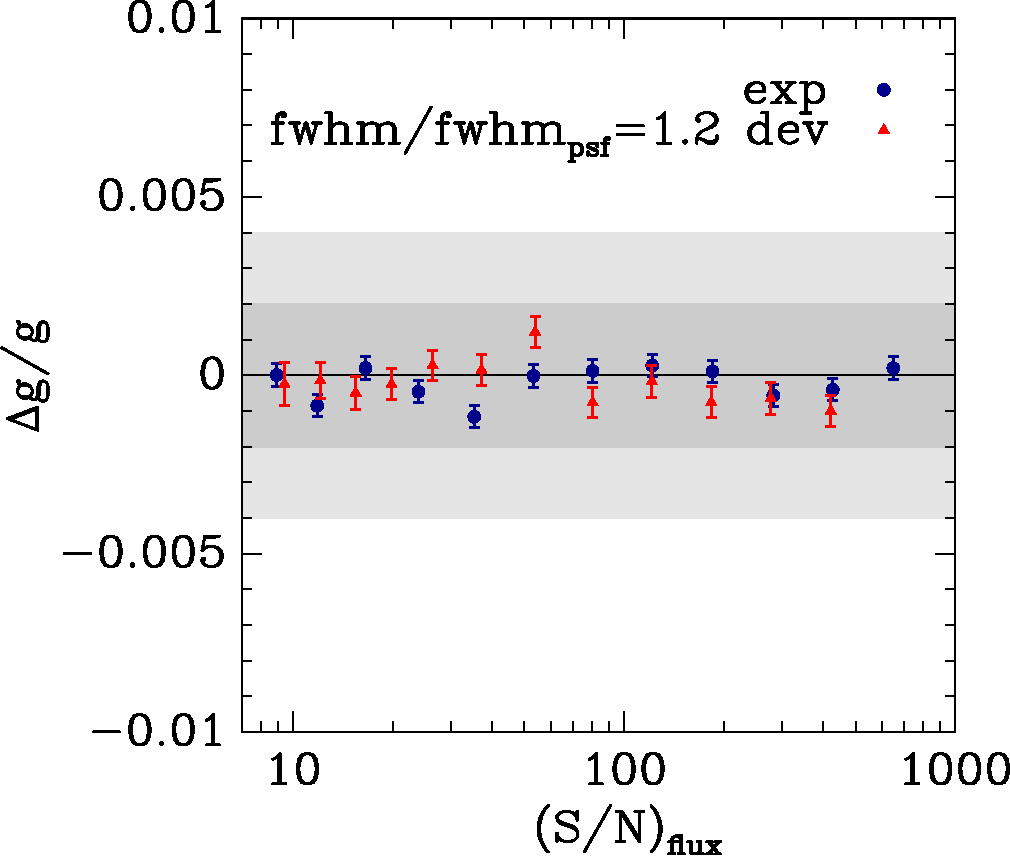
\includegraphics[width=\textwidth]{ngmix-flux-s2n-sigrat-20.pdf}
            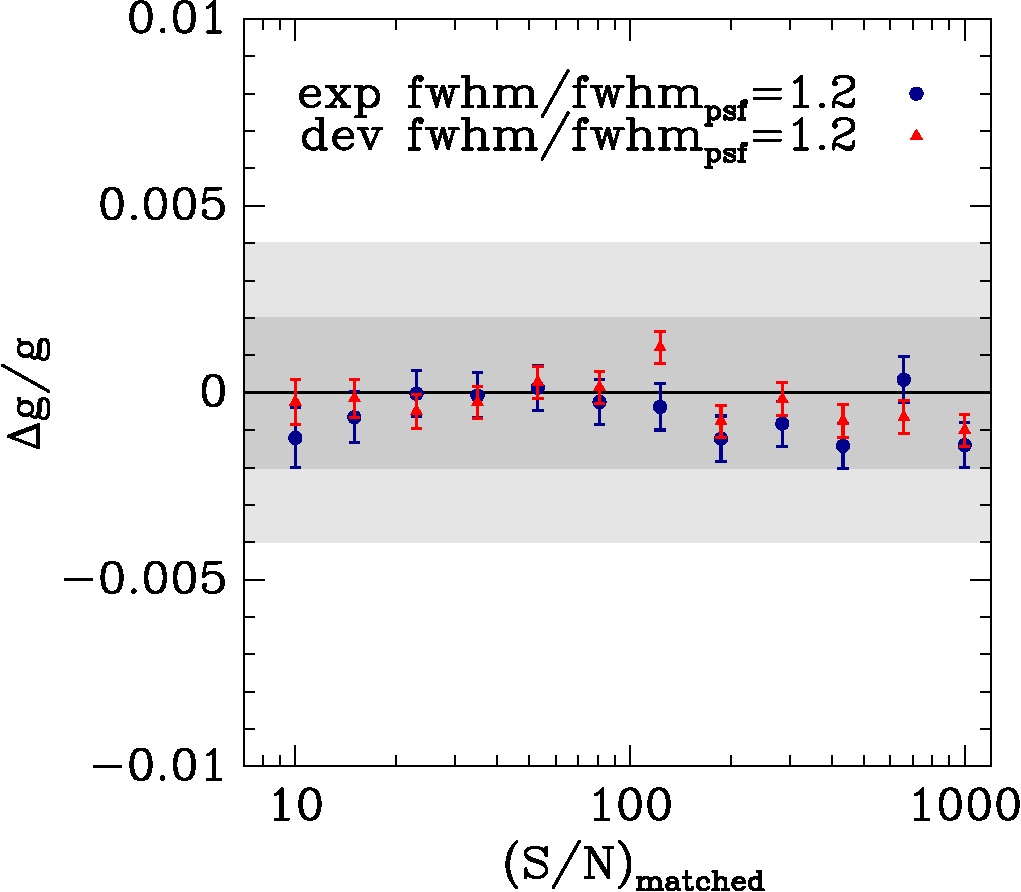
\includegraphics[width=\textwidth]{ngmix-fwhm12.pdf}
            \newline

        \end{column}
    \end{columns}

}

\frame
{
    \frametitle{Erin Sheldon: Multi-epoch data processing}

    \begin{itemize}
        \item Each patch of sky is typically visited more than 10 times
            by DES (hundreds by LSST)
        \item Each epoch has a different point spread function.   Simply adding
            them results in PSF discontinuities, bizarre PSF shape. 
        \item Better way is to analyze all the epochs simultaneously.
        \item E.S. Created a new data structure holding ``postage stamps''
            for all epoch associated with every object.
        \item E.S. and others now using these multi-epoch data structures (MEDS) to 
            process DES data.
        \item Translates directly to LSST.
    \end{itemize}
}

\frame
{
    \frametitle{Erin Sheldon: Multi-epoch data processing}

    \begin{center}
        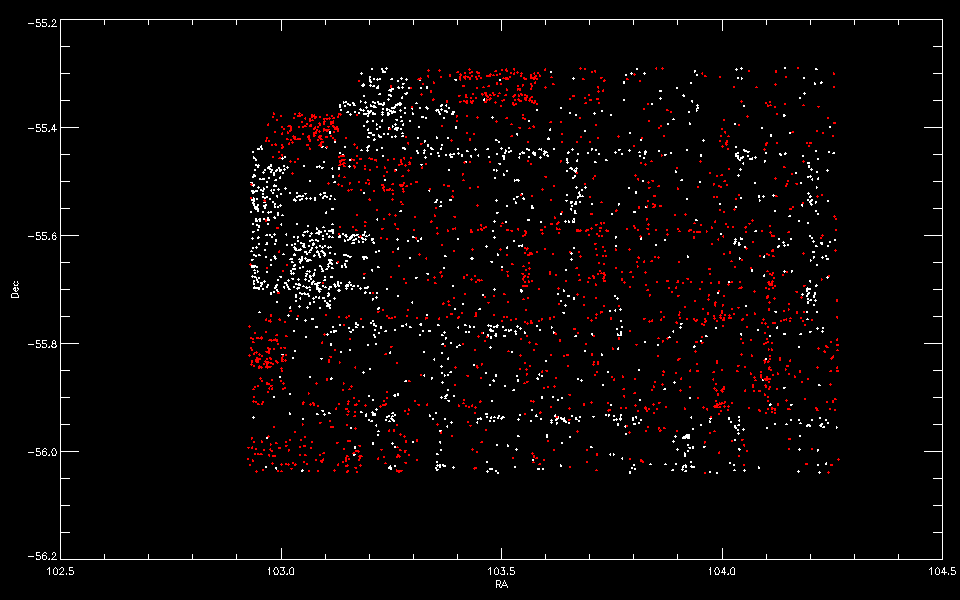
\includegraphics[width=0.7\textwidth]{delta_psf_pos.png}
    \end{center}
    \fontsize{9}{0.8\baselineskip}
    \begin{itemize}
        \item Difference in brightnesses of stars measured using
            multi-epoch fitting versus standard ``coadd'' of images.
        \item linear features are due to discontinuities in the
            point spread function at chip boundaries: the 
            brightness measured in the coadd is wrong.
    \end{itemize}
}


\frame
{
    \frametitle{Erin Sheldon: Multi-epoch data processing}

    \begin{itemize}

        \item E.S. measuring star and galaxy photometry and 
            lensing shear using MEDS files.

        \item Photometry performing significantly better than
            standard analysis.

        \item Inital shear measurements running now.  Should have a full
            processing of early data in the next month.

    \end{itemize}
}



\frame
{
    \frametitle{Andres Plazas: DES Detector Characterization}

    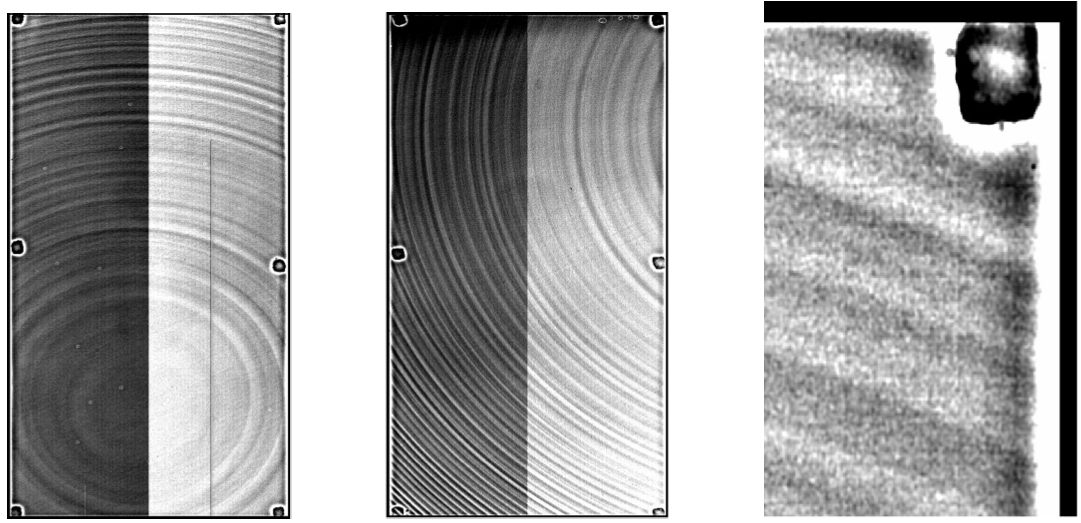
\includegraphics[width=\textwidth]{flats.png}
    \newline

    \begin{center}
        Tree rings and tape bumps in a flat field image.
    \end{center}
} 
\frame
{
    \frametitle{Andres Plazas: DES Detector Characterization}

    \fontsize{9}{0.7\baselineskip}
    \begin{columns}
        \begin{column}{0.4\textwidth}
            \begin{itemize}

                \item Tree-rings are features in the CCDs that occur during
                    fabrication.  Variations in doping produces a spurious
                    transverse electric field, changing the effective location
                    and area of each pixel.

                \item In typical image reduction the data are divided by these
                    calibration frames, but this is incorrect : our
                    measurements indicate this introduces large systematic
                    errors.

                \item We measure these instrumental signatures and produce
                    models that fit the data well.

            \end{itemize}
        \end{column}
        \begin{column}{0.6\textwidth}
            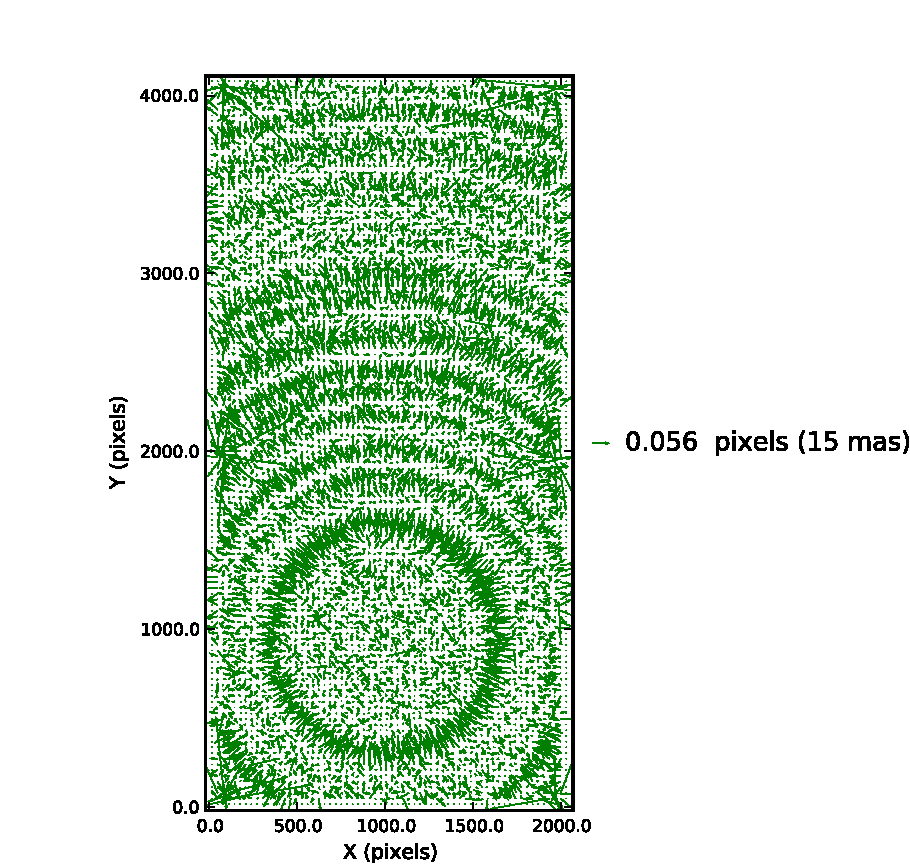
\includegraphics[width=\textwidth]{N22_astrometric_single-crop.pdf}
            \newline

            {\tiny Astrometric residuals from polynomial model caused by
            the ``tree rings''. \par}


        \end{column}
    \end{columns}


}

\frame
{
    \frametitle{Andres Plazas: DES Detector Characterization}

    \begin{center}
    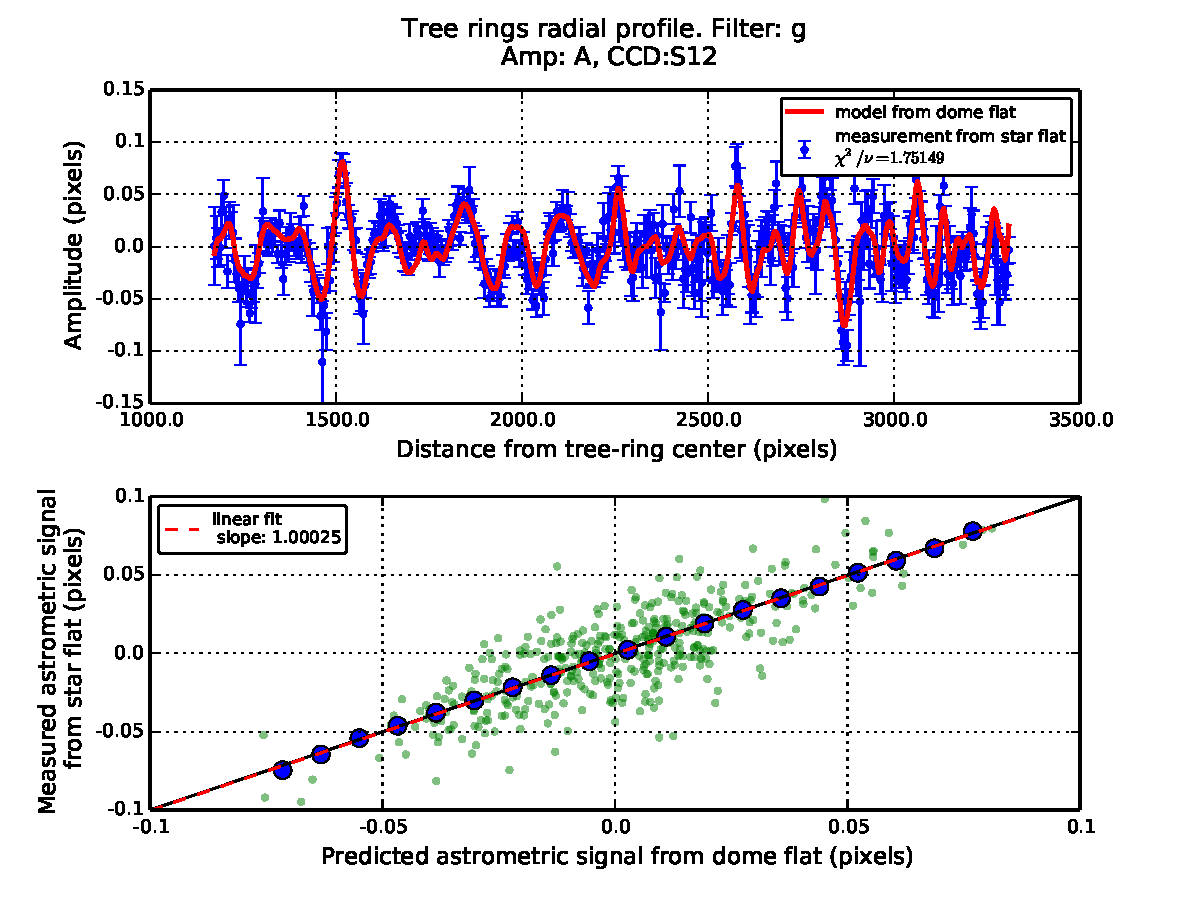
\includegraphics[width=0.7\textwidth]{astrometric_residuals_vs_model_S12.pdf}
\end{center}

    \fontsize{9}{0.8\baselineskip}
        \begin{itemize}
            \item Astrometric residuals binned in radius from center of tree ring.
            \item Prediction from model fit to the flat field matches well.
            \item Model will be incorporated into all DES analyses.  Simple
                to include in multi-epoch image processing.
            \item Accepted for publication in PASP.  arXiv:1403.6127
        \end{itemize}
}

\frame
{
    \frametitle{E.S. and A.P: Preliminary Cluster Lensing Results}

    \fontsize{9}{0.8\baselineskip}
    \begin{columns}
        \begin{column}{0.4\textwidth}    
            \begin{itemize}
                \item RedMapper clusters in early DES data.
                \item Signal binned by cluster richness $\lambda$.
                \item Detection in all bins.
                \item Plenty of signal!
            \end{itemize}
        \end{column}
        \begin{column}{0.6\textwidth}
            \begin{center}
                \includegraphics[width=\textwidth]{binned-rmdes01im3shape-r01-lambda-12-allplot.pdf}
                \newline
                Preliminary
            \end{center}
        \end{column}
    \end{columns}
}

\frame
{
    \frametitle{Summary}

    %\fontsize{9}{0.9\baselineskip}
    \begin{itemize}

        \item DES data is in hand.

        \item E.S. producing improved shear catalog and improved photometry.
        \item A.P. characterized detectors, will be included in all DES analyses.
            
        \item E.S. and A.P. preliminary lensing measurements of galaxy clusters.

    \end{itemize}
}



\end{document}
